\section{Instrumenting applications}
\label{sec:applications}

The PTT framework reduces the process of instrumenting an application to three
steps:

\begin{enumerate}
\item Integrate the source into the build system.
\item Define the partial PCF files.
\item Insert the API calls in the code.
\end{enumerate}

This process can be shortened even more, because the second step is optional.
But tu illustrate it completely, the rest of the section is explains the details
with the aid of a real example: the \emph{blackscholes} benchmark, from the
PARSEC suite.

The PTT dependencies for compilation are:

\begin{itemize}
\item GNU make.
\item GNU C compiler and linker.
\item A minimal UNIX environment, including some implementation of AWK
available.
\end{itemize}


\subsection{Build system integration}

The \emph{blackscholes} application consists of one source file, therefore
compiling it is straight forward.  For simplicity, the source is contained in
the directory \verb:parsec: and the tracing library source is reachable by
following the relative path \verb:../ptt/tracelib:.  Then, the first step is to
create a \verb:Makefile:.  The contents are listed in listing
\ref{code:makefile1}.

\begin{listing}
\label{code:makefile1}
\caption{A simple \texttt{Makefile}}
\begin{verbatim}
  PTT_PATH := ../ptt/tracelib
  PROGRAMS := blackscholes
  blackscholes_SOURCES := blackscholes.c
  blackscholes_LIBS := m

  include $(PTT_PATH)/rules.mk
\end{verbatim}
\end{listing}

That is the minimum build rules necessary to generate instrumented binaries.
The first, second and last lines are mandatory, otherwise the build system does
not know what to build nor where to find the tracing library.  It is possible to
have many binaries handled by the same \verb:Makefile:; but for each of the
listed programs, the \verb:program_SOURCES: variable needs to be specified.
Note that header files can also be included in it, and it will provide more
dependency information.  For example, suppose there was another application in
the same directory as the example, the \verb:Makefile: would then look like
listing \ref{code:makefile2}.

\begin{listing}
\label{code:makefile2}
\caption{A \texttt{Makefile} to handle multiple programs}
\begin{verbatim}
  PTT_PATH := ../ptt/tracelib
  PROGRAMS := blackscholes otherprog
  blackscholes_SOURCES := blackscholes.c
  blackscholes_LIBS := m
  otherprog_SOURCES := main.c module.c module.h

  include $(PTT_PATH)/rules.mk
\end{verbatim}
\end{listing}

Also for each program specified in the \verb:PROGRAM: variable, it is possible
to define a \verb:prog_LIBS: and \verb:prog_PCF: variables.  The former is a
list of libraries needed at link time.  In the example, \emph{blackscholes}
needs the math library (\verb:-lm: compiler switch).  Note that it is not
necessary to explicitly specify the linkage against the \emph{PThreads} library,
as it it assumed by the build system.  The latter will be explained later on.

At this stage, it is already possible to compile running just \verb:make:.  It
generates a binary called \verb:blackscholes: which, after each execution,
generates three files named \verb:ptt-trace-000:\footnote{The last numbers are
incremented to preserve already existing files} with extensions ``\verb:.prv:'',
``\verb:.pcf:'' and ``\verb:.row:''.  These are the files needed by Paraver to
visualize a trace.

\begin{figure}
\centering
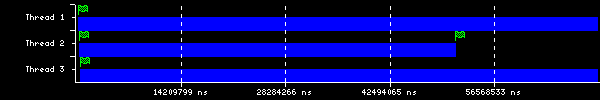
\includegraphics{pics/bs-stage1.png}
\caption{Resulting trace with no manual instrumentation}
\label{fig:bs-stage1}
\end{figure}

So, with no modification in the source code yet, the binary generates traces
containing minimal information about thread creation, destruction and eventual
event flushing operations.  Figure \ref{fig:bs-stage1} shows an example.


\subsection{Event definition}
\label{sec:pcf_sample}

Although this step is optional, it can become very helpful when manipulating
resulting traces.  The purpose is to enhance the human readable event
information provided to Paraver.

The idea is to write directly a \textbf{partial} PCF\footnote{\emph{Paraver
Configuration File}} file, or multiple files.  That is, write event and value
definitions that will be appended to the basic PCF file, provided by the
framework.

In the example, a \emph{Phase} event could be defined, with several possible
values:

\begin{listing}
\label{code:pcf1}
\caption{A simple PCF file}
\begin{verbatim}
  EVENT_TYPE
  0    7000    Phase
  VALUES
  0      None
  1      Running
  2      Mutex wait
  3      Critical section
  4      Barrier wait
\end{verbatim}
\end{listing}

Now it is necessary to acknowledge the existence of this new file to the build
system.  Therefore, listing \ref{code:makefile1} should be changed to what is
shown by listing \ref{code:makefile3} following, assuming that listing
\ref{code:pcf1} is saved as \verb:blackscholes.pcf:.

\begin{listing}
\label{code:makefile3}
\caption{Second step for the simple \texttt{Makefile}}
\begin{verbatim}
  PTT_PATH := ../ptt/tracelib
  PROGRAMS := blackscholes
  blackscholes_SOURCES := blackscholes.c
  blackscholes_LIBS := m
  blackscholes_PCF := blackscholes.pcf

  include $(PTT_PATH)/rules.mk
\end{verbatim}
\end{listing}

The way events are organized in different files is quite flexible.
Nevertheless, in the end all specified PCF files are concatenated and processed
altogether.  In particular, the variable \verb:PCF_FILES: provides a way to
share a PCF file among all the programs controlled under the same
\verb:Makefile: without having to explicitly add it to each \verb:prog_PCF:
variable.  For example, in order to share the PCF described in listing
\ref{code:pcf1} with all the other programs, an example using the
\verb:PCF_FILES: variable is illustrated by listing \ref{code:makefile4}.

\begin{listing}
\label{code:makefile4}
\caption{Multiple program \texttt{Makefile} sharing a PCF file}
\begin{verbatim}
  PTT_PATH := ../ptt/tracelib
  PROGRAMS := blackscholes otherprog
  PCF_FILES := blackscholes.pcf
  blackscholes_SOURCES := blackscholes.c
  blackscholes_LIBS := m
  otherprog_SOURCES := main.c module.c module.h

  include $(PTT_PATH)/rules.mk
\end{verbatim}
\end{listing}

From here, the build system automatically provides as many derived constants as
events and values defined in all specified PCF files.  The names, though, are
mangled a bit by replacing spaces with underscores and transforming all the
letters to uppercase.  For example, the previous PCF listing would provide the
following constants at compilation time:

\begin{itemize}
\item \verb:PHASE:
\item \verb:NONE:
\item \verb:RUNNING:
\item \verb:MUTEX_WAIT:
\item \verb:CRITICAL_SECTION:
\item \verb:BARRIER_WAIT:
\end{itemize}


\subsection{Inserting events}

Finally, it is time to insert the interesting events to investigate after the
executions, directly from Paraver.  There are two functions, already available
from the build system, that generate events:

\begin{verbatim}
  void ptt_event  (int type, int value);
  void ptt_events (int count, int type1, int value1, ...);
\end{verbatim}

In fact, these are the only functions available to the user.  The reason for the
second function to exist is to provide the ability to generate multiple events
with the exact same time value.  Once instrumented, the binary will generate the
proper files to be interpreted by Paraver.

Note that the instrumented binaries can generate traces with a prefix other than
\verb:ptt-trace: in their filenames.  By setting the \verb:PTT_TRACE_NAME:
environment variable, its contents will be used as a trace filename prefix
instead of the default.

% vim:ft=tex:spell
